\section{Cerberus and Optimization Enhancement}
\label{Sec:Scheduler}

\subsection{Cerberus for 3-Phase Jobs}
Traditional batch scheduler usually looks at the field of $c_i$ and $rt_i$
when making scheduling decision.
One straightforward way to make decisions on non-burst-buffer HPC system is
First Come First Serve, as long as available compute nodes can satisfy user job.
Once the system is equipped with burst buffer, scheduler must consider a new constraint:
the available amount of burst buffer capacity.
Scheduling is divided into 3 phases to
adopt to the 3-phase characteristic of jobs in burst buffer context.
As shown in Figure~\ref{Fig:CerberusQueues},
Cerberus schedules jobs in 3 distinct set/queue.
The input queue $Q_I$ contains all the jobs that
needs to load input data before they are able to execute.
Once a job comes out of input queue, its data flows from external disk
to burst buffer nodes and then to memory on compute nodes.
At this moment, compute nodes are not allocated to the application yet.
The run queue $Q_R$ contains all the jobs waiting to be run with loaded data.
When running application request checkpointing, its execution and data are
pushed to its exclusive burst buffer nodes;
when application resume from system fault, its checkpointing are
loaded directly from burst buffer, instead of PFS, to compute nodes.
The output queue $Q_O$ contains all the jobs that
terminate execution but needs to write output data to external storage.
Compute nodes are released by the applications in this phase;
in other words, other applications ready to run can take up them now.
At anytime, a job can only appear in one of the 3 sets, apparently.
This fact motivates separated scheduling idiom to be used in different phases,
or for different job queues.

%\begin{figure}[!t]
        %\centering
        %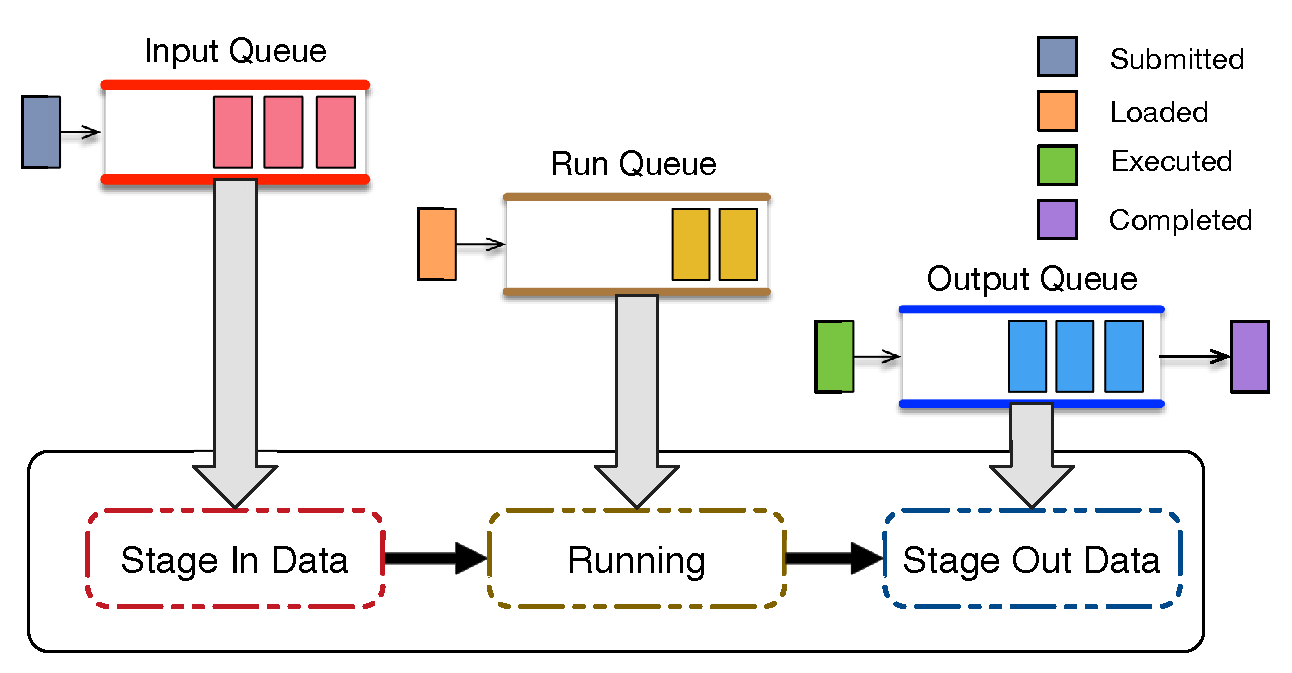
\includegraphics[width=3.6in]{CerberusQueues}
        %\caption{Scheduling Process of Burst Buffer Aware Cerberus}
        %\label{Fig:CerberusQueues}
%\end{figure}

\begin{figure}[!t]
        \centering
        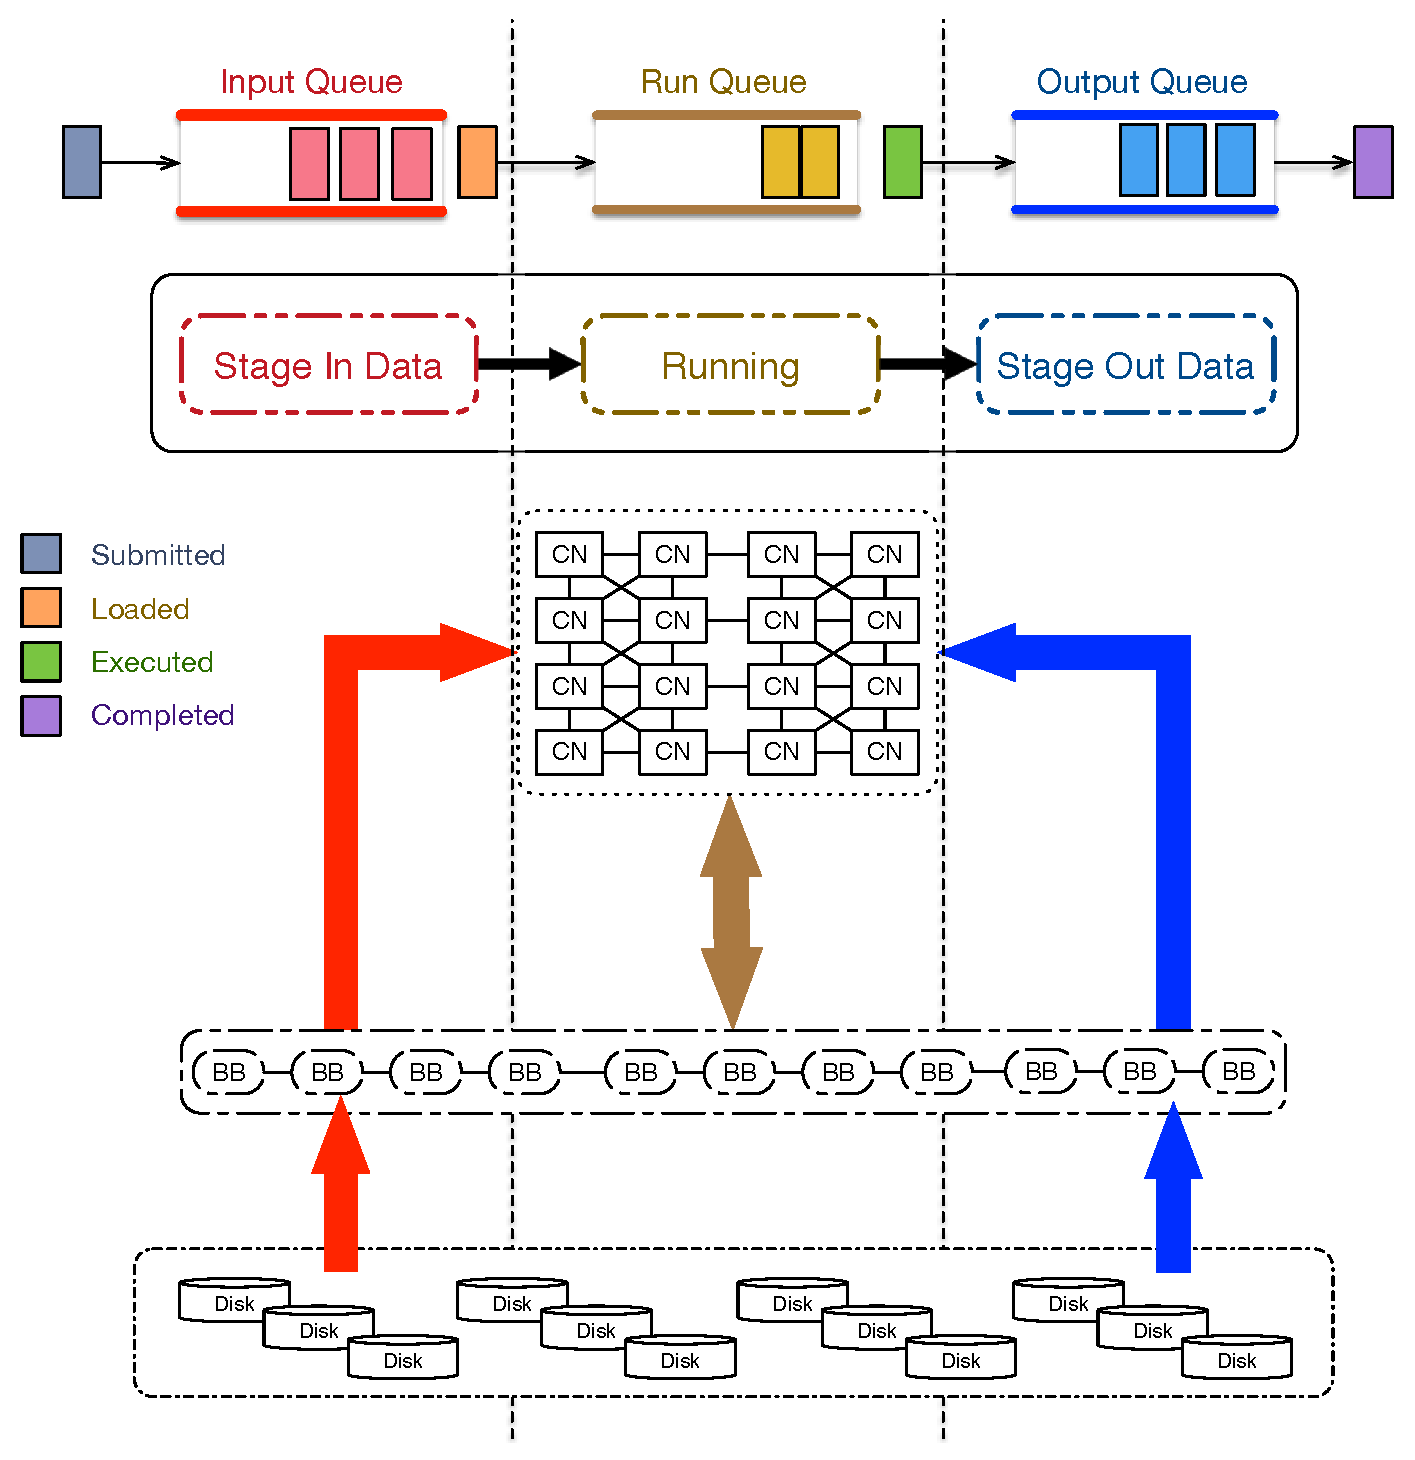
\includegraphics[width=3.6in]{CerberusBBSystem}
        \caption{Scheduling Workflow of Cerberus}
        \label{Fig:CerberusQueues}
\end{figure}


\subsection{Optimize Stage-In Phase}
In the stage-in phase, only burst buffer demand is considered.
Scheduling are made based on the value of $bb\_in$ of jobs in $Q_I$.
If we care about data transfer throughput,
we should transfer as much data as possible by doing the following optimization:
\begin{align*}
        & \max \sum_{i\in S} bb\_in_i \textit{   s.t.}\\[1em]
        & \left\{
                \begin{array}{l}
                        S \cup NS = J \\ [1em] \numberthis \label{Equ:MaxTransferData} 
                        \sum_{i\in S} bb\_in_i \leq BB_{available}
                \end{array} 
        \right.
\end{align*}	

If we care about task parallelism, following optimization could help:
\begin{align*}
        & \max |S| \textit{   s.t.} \\[1em]
        & \left\{
                \begin{array}{l}
                        S \cup NS = J \\ [1em] \numberthis \label{Equ:MaxTaskNumber} 
                        \sum_{i\in S} bb\_in_i \leq BB_{available}
                \end{array} 
        \right.
\end{align*}
The number of tasks doing data loading will be maximized.


\subsection{Optimize Running Phase}
Running jobs require not only compute nodes, but burst buffer to ensure performance and correctness.
Scheduling are accordingly made based on the value of $c$ and $bb\_run$ of jobs in $Q_R$.
To maximize multiple types of resource's utilization,
we convert it to the knapsack problem by defining the value of the $job_i$ as
\begin{equation}
        v_i = \frac{c_i / CN}{rt_i} \times \frac{bb\_run_i / BB}{rt_i}
        \label{Equ:DefValue}
\end{equation}
where $rt_i$ is the running time of $job_i$, the time it takes up the computing nodes.
By defining \textit{value} as Equation~\ref{Equ:DefValue},
we prefer these tasks that claims to take up node resources with short duration.
Unfortunately, it is difficult to predict $rt_i$ before actually running the job.
Of course we could use the \textit{expected running time} $ert_i$ specified by user.
However, by examining the log traces from ANL\cite{JobTrace},
we found that the variance between $rt_i$ and $ert_i$ is significantly different.
For now we can just assume $rt_i$ is constant for all jobs.
In the future, we could adopt machine learning or data mining ideas to predict the running time of a job with demand vector.
Notice that then the value of a task is proportional to $c_i*bb_i$.
The optimizing formula can thus be
\begin{align*}
        & \max \sum_{i \in S}c_i * bb\_run_i \textit{   s.t.}\\[1em]
        & \left\{
                \begin{array}{l}
                        S \cup NS = J \\ [1em]
                        \sum_{i \in S} c_i \leq CN_{available} \\ [1em] \numberthis \label{Equ:MaxProduct} 
                        \sum_{i \in S} bb\_run_i \leq BB_{available}
                \end{array} 
        \right.
\end{align*}


\subsection{Optimize Stage-Out Phase}
Scheduling are made based on the value of $bb\_out$ of jobs in $Q_O$.
Optimization formula for different purpose are almost the same as these in IO-BB scheduling.


\subsection{Solving the Optimization Problems}
It is trivial to show that optimization problem~\ref{Equ:MaxTransferData}
and~\ref{Equ:MaxTaskNumber}
are equivalent to 0-1 knapsack problem.
Problem~\ref{Equ:MaxProduct} can be informally treat as two dimension 0-1 knapsack problem.
In fact, we expect all of them are NP-hard problems.
We can solve them with dynamic programming in pseudo polynomial time.
Applying memorization could also help accelerate the solving process.
In fact we are not interested in the optimal result of problem~\ref{Equ:MaxTransferData},
problem~\ref{Equ:MaxTaskNumber} and problem~\ref{Equ:MaxProduct} at all
but in a combination of jobs that yields the optimal solution,
which can also be easily tracked back down by keeping memorizations.

Since problem~\ref{Equ:MaxTransferData},
problem~\ref{Equ:MaxTaskNumber} and problem~\ref{Equ:MaxProduct} are very similar, 
their solution is also highly related.
First, for problem~\ref{Equ:MaxTransferData}, the recursive relationship is
given by Recursion~\ref{Equ:MaxTransferDataRecursion}.
In~\ref{Equ:MaxTransferDataRecursion}, the memo we keeps during solving is
the optimal solution for 
$jobs=(job_1, job_2, \ldots, job_i)$ with $w$ GB of available burst buffer.
It turns out that the recursion for problem~\ref{Equ:MaxTaskNumber} is
extremely similar to~\ref{Equ:MaxTransferDataRecursion}
The memo in Recursion~\ref{Equ:MaxTaskNumberRecursion} is the same
as that in Recursion~\ref{Equ:MaxTransferDataRecursion}.
The recursion for problem~\ref{Equ:MaxProduct} is a little bit complicated.
Here we should keep the memo of the optimal solution for $jobs=(job_1, job_2, \ldots, job_i)$
with $c$ computing nodes and $w$ GB of burst buffer being available.

Scheduler can obtain an optimal combination of jobs by examining the memo.
Take the problem~\ref{Equ:MaxProduct} problem for example.
We start from $dp(n, CN, BB)$.
If $c_n \leq CN$ and $bb\_in_n \leq BB$, $job_n$ should be scheduled if
$dp(i-1, c, w) \leq dp(i-1, c - c_i, w - bb\_in_i) + c_i bb\_in_i$ and
recurse with $dp(n - 1, CN - c_i, BB - bb\_in_i)$;
otherwise, $job_n$ should be skipped and we recurse the process on $dp(n-1, CN, BB)$.
The time complexity of solving Equation~\ref{Equ:MaxTransferDataRecursion} and
Equation~\ref{Equ:MaxTaskNumberRecursion} is $O(n\times BB)$.
The time complexity of solving Recursion~\ref{Equ:MaxProductRecursion}
is $O(n\times CN\times BB)$.
Notice that $CN$ and $BB$ may be very large integers,
making the pseudo-polynomial algorithm unsuitable
to be used online by scheduler.
In practice, we could reduce the time complexity by allocating resource
in a coarser granularity.
For example, jobs usually asks for compute node in the unit of 512 nodes;
its demand for burst buffer nodes usually in the unit of 100 GB.
Then we could divide both $CN$ and $c_i$ by 512;
divide both $BB$ and $bb\_in, bb\_run, bb\_out$ by 100.
It is also possible to reduce the value of $n$, the number of jobs in the queue.
For example, whenever we more resources,
we can consider only $\frac{1}{\alpha}n$ jobs in the queue.
This will give us only the partial optimal solution in exchange of less computation complexity.



\begin{strip}
        \begin{align}
                dp(i, w) = & 
                \left\{
                        \begin{array}{l}
                                0, \text{ if $i=0$ } \\ [1em]
                                dp(i-1, w), \text{ if $bb\_in_i > w$} \\ [1em]
                                \max \{ dp(i-1, w), dp(i-1, w-bb\_in_i) + bb\_in_i \}, \text{ if $bb\_in_i \leq w$}
                        \end{array} 
                \right.
                \label{Equ:MaxTransferDataRecursion} 
        \end{align}
\end{strip}

\begin{strip}
        \begin{align}
                dp(i, w) = &
                \left\{
                        \begin{array}{l}
                                0, \text{ if $i=0$ } \\ [1em]
                                dp(i-1, w), \text{ if $bb\_in_i > w$} \\ [1em]
                                \max \{ dp(i-1, w), dp(i-1, w-bb\_in_i) + 1 \}, \text{ if $bb\_in_i \leq w$}
                        \end{array} 
                \right.
                \label{Equ:MaxTaskNumberRecursion}
        \end{align}
\end{strip}


\begin{strip}
        \begin{align}
                dp(i, c, w) = &
                \left\{
                        \begin{array}{l}
                                0, \text{ if $i=0$ } \\ [1em]
                                dp(i-1, c, w), \text{ if $c_i > c$ or $bb\_run_i > w$} \\ [1em]
                                \max \{ dp(i-1, c, w), dp(i-1, c - c_i, w - bb\_run_i) + v_i \}, \text{ if $c_i \leq c$ and $bb\_run_i \leq w$}
                        \end{array} 
                \right.
                \label{Equ:MaxProductRecursion}
        \end{align}
\end{strip}

